\documentclass{standalone}
\usepackage[T1]{fontenc}
\usepackage[utf8]{inputenc}
\usepackage[english]{babel}
\usepackage{tikz}
\usetikzlibrary{calc,through,backgrounds,positioning,fit}
\usetikzlibrary{shapes,arrows,shadows}

\begin{document}

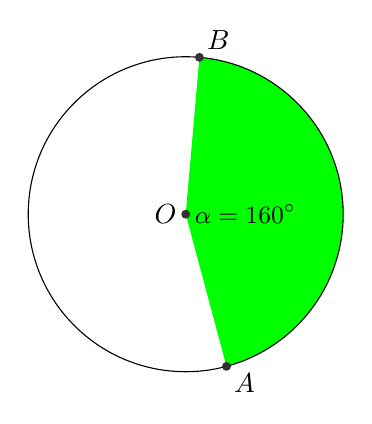
\begin{tikzpicture}[scale=1,inner sep=0.4mm]
\fill[green] (0,0) -- (2cm,0) arc (0:85:2cm) -- cycle;
\fill[green] (0,0) -- (2cm,0) arc (0:-75:2cm) -- cycle;
\coordinate (O) at (0,0);
\coordinate (A) at (-75:2cm);
\coordinate (B) at (85:2cm);
\draw (0,0) circle (2cm);
\node at (O) [circle,fill=black!80!white] {};
\node at (A) [circle,fill=black!80!white] {};
\node at (B) [circle,fill=black!80!white] {};
\node at (O) [left=2pt] {$O$};
\node at (A) [below right=2pt] {$A$};
\node at (B) [above right=2pt] {$B$};
\node at (O) [right=2pt] [font=\small]{$\alpha=160^{\circ}$};
\end{tikzpicture}

\end{document}
